\documentclass{article}
\usepackage[english]{babel}
\setlength{\parindent}{24pt}
\usepackage{indentfirst}
\usepackage{graphicx}
\usepackage{setspace}

\doublespacing
\newcommand{\BibTeX}{{\sc Bib}\TeX}

\begin{document}

\title{Final Report}
\author{Qi Mao\\
  \texttt{maoxx241@umn.edu}
  \and
  Haowen Luo\\
  \texttt{luoxx560@umn.edu}
  }
\maketitle

\section{Abstract}
Machine learning become a vital part of crime detction. In this research, We use scikit-learn, a free software machine learning library, to conduct a cojmparative study between location of crime and the type of crime. The ata for the City of Chicago that has been provided by catalog.data.gov. We implemented the Random Forest, Logistic Regression, Naive Bayes, abd Decision Tree algorithms using the same finite set of features, on the crime dataset. Overall, the Logistic Regression algorithm and Random Forest performed the best among the four selected algorithms. The purpose of this project is to prove how accurate the machine learning algorithms can be at predicting the type of crime based on location desription.

\section{Description}
As international students, the safety of us is always the most problem concerned by our parents. So, we would like to build a model to help them understand what situation of crime in the major cities of the United States. The purpose of this project aims to discuss the relationship between the type of crime and the area of Chicago. Why is Chicago? As one of the biggest and most developed cities in the Midwest of the United States, Chicago is representative. And it is a well-known city near Minneapolis which means more persuasion for parents of international students. For another important reason, the Chicago Data Portal provides the most detailed and reliable data to analysis on the website. This model we build should not only provide clear and visualized information to parents but also help the police to predict what kinds of crime happened in this area after they receive a report. So, a reliable source data is necessary. To build a model with practicality, the result’s accuracy of our model wouldn’t be neglected, and it is also an important parameter to check the usability and reliability of our model. More detail we will discuss in follow contents.

\section{background}
Crime is always an important social security problem for every country. However, it can be studied and analyzed by using many different methods as Patricia L. Brantingham claimed.\cite{brantingham1998mapping} Then we build a model with some algorithm to review the record of crime in a region and analysis it. What specific problem we should focus on is the next problem. “Crime cannot be predicted since it is neither systematic nor random.”, said by Shiju Sathyadevan.\cite{sathyadevan2014crime} However, Mr. Sathyadevan thinks crime prevention is a systematic method for identifying what kinds of crime happening. That is support for our crime prediction project. We think crime prediction would be very useful for social security department to prevent crime or protect the safety of officers. For this project, we would like to use Random Forest, Logistic Regression, Naive Bayes and decision tree. We will discuss them in detail in the description part. “USING MACHINE LEARNING ALGORITHMS TO ANALYZE CRIME DATA” is a good example project which analyzes the data of the FBI's Uniform Crime Reporting (UCR) program.\cite{mcclendon2015using} We think it would be an example for inspiring us to finish our project by step and step.

Logistic Regression was used to classify individuals in the target categories based on the logistic function and it forces estimated probabilities to lie within the range 0-1, which is more sensible than linear regression.\cite{liu2011comparison}
In Liu's paper, he builds three models for predicting violent re-offending. They provided the accuracy and AUC range of the three models. And they provided that the NNs was slightly better Than that Logistic Regression model, it did not demonstrate a significant improvement.

Random Forest can have profound effects on prediction quality as well as the to be introduced variable importance measures.\cite{chen2016events}. In Chen's paper, he used the random forest to find the most important features. And they provided that the random forest can find several expected related features. We can use that to find something interesting.

Naive Bayes has the ability to predict the probability that a given tuple belongs to a particular class.\cite{iqbal2013experimental} They also mentioned that if talking about solving complex classification problems, then naive bayes is not a recommended choice. In our project, we will clean up the data and make the question simple. So we can use Naive Bayes that can short training time and fast evaluation.

"we classify crime data using decision tree into two classes, such as danger and neutral.", said by Nasridinov. \cite{nasridinov2013decision} They provided that decision tree can analyze are good enough to motivate us to use a decision tree in order to predict future crimes. So we can also try to simplify our question that we only consider the question only have two classes.

"An ROC curce is useful for comparing the relative performance among different classifiers."\cite{Tan:2018:IDM:3208440} And precision and recall are also widely used metrics employed. In our project, we will use them to compare which classifier has the best performance.

\section{Approach}
In our dataset, crimes are documented in details with time, latitude, longitude, location description, and crime type. We draw a map by random sampling to find the information we need.
We will find the top 11 typical crime types through plotting. Then we will simplify the problem, remove the features we don't need, and remove missing values. Then, we will handle our location description feature to facilitate the next steps. Then we will use three to seven ratios to split test data and train data.

After the preparation is complete, we will import 4 models via the scikit-learn library. and training models

Finally, we will choose four models to evaluate the dataset and find the relationship between the type of crime and the location of the crime. We will choose the Decision Tree, Naive Bayes, random forest, and  Logistic Regression. According to the accuracy, precision, and recall, we will show the performance of each model. and we will plot the ROC curve of each model. From the random forest, we can find the feature importance. 

\section{experiment}
First we import the data and draw the scatter plot of the main crime types. We can see that from 2001 to 2018 the main types of crime are theft and battery. We found some interesting information through the map. We randomly sampled the crime with the crime type of theft and battery, and plotted the sample on the map based on latitude and longitude.
\begin{figure}
    \caption{This is map of theft}
    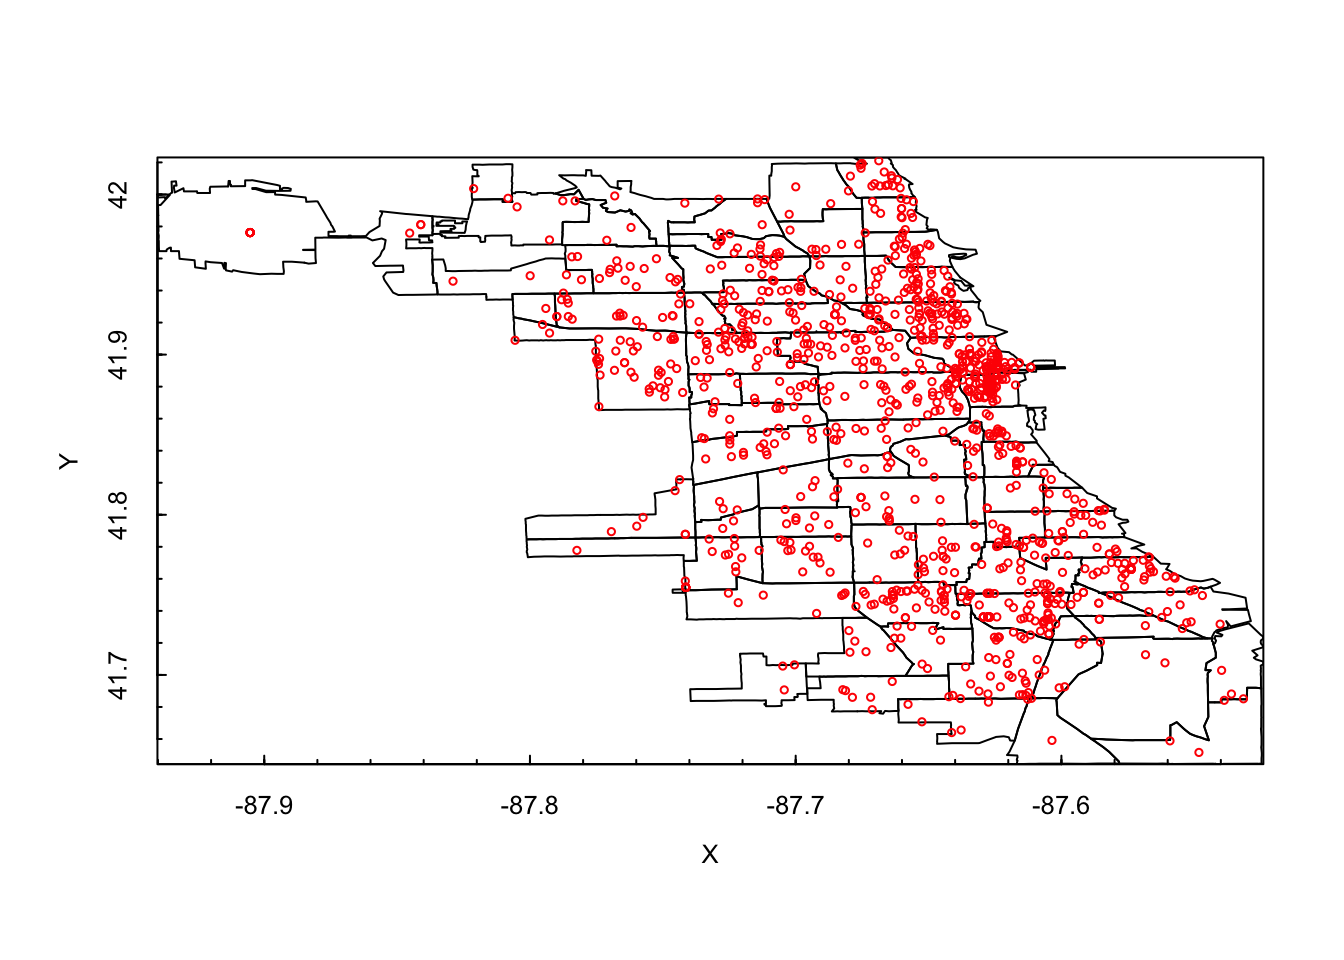
\includegraphics[scale=0.25]{theft}    
\end{figure}

\begin{figure}
    \caption{This is map of battery}
    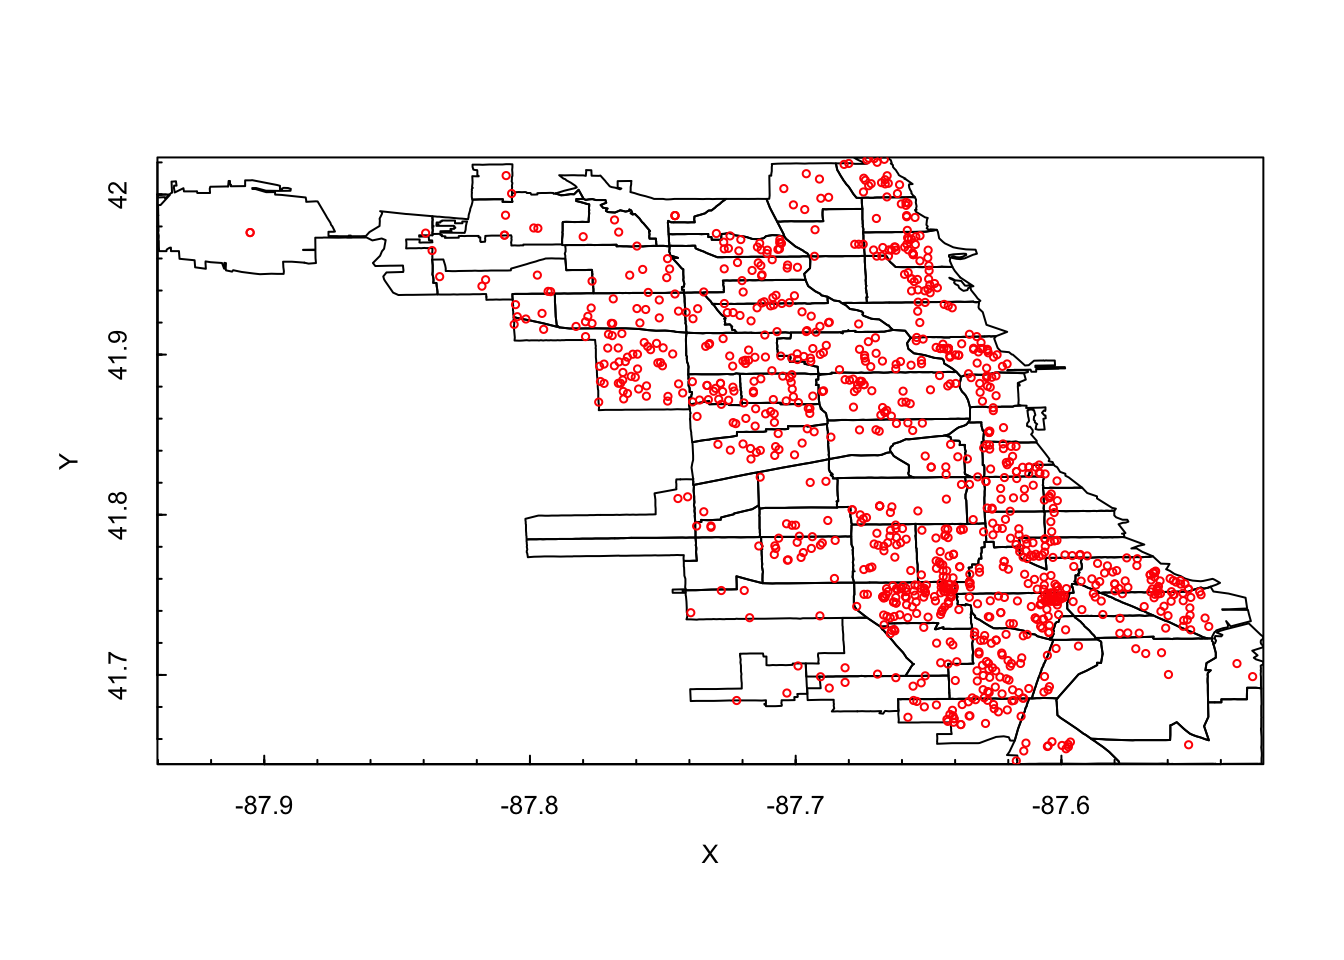
\includegraphics[scale=0.25]{battery}
\end{figure}

Through two maps, we can clearly find out that the main areas where theft and battery crimes are different are different. The main area of theft is in the northeast, while the main area of the battery is in the south. We can determine the relationship between crime type and latitude and longitude.

For the data clean up, we drop columns we are not using first. Thoung there are many features in this dataset, some information are not useful such as ID. We want to focus on the relationship between location and crime type, so we only need latitude and longitude and location description. Then we remove missing data. location description feature is categorical data, we converted it to dummy variables. 

In order to simplify the problem to two classification problem, we decided to study only two main types of crime. In the previous study, we found that there is a clear correlation between the two types of crimes and location.

We have a baseline model that the theft crime accounts for 51$\%$ of the total sample, while battery is around 49$\%$. An acceptable model should have at least have the baseline accuracy of 51$\%$.

We build the Random forest model first. Because we can get the feature importance from this model. Random forest's accuracy is 0.73, and the precision is 0.71, the recall is 0.74, which is a good performance model. By exporting the feature importance, we can see whether, in addition to the latitude and longitude, whether the location of the case is in an apartment or a store is an important feature to confirm whether the type of the case is theft.

We build the Logistic regression model next. We can use the 10-fold cross validation to conclude that our model is generalizing well or not. After fitting the model, we obtained a model with an accuracy of 0.73, and the average accuracy of 10-fold cross validation was also 0.725. We can conclude that our model generalizes well. Both precision and recall are 0.72.

Next, we use Naive Bayes and decision tree, both of which have good performance in other crime type prediction cases. For Naive Bayes model, the accuracy is 0.65, the precision is 0.59, but the recall is 0.92. A low precision essentially means that the classifier returns a lot of false positives. Naive Bayes has the worst performance among the four models. The decision tree's accuracy, precision, and recall are all at an acceptable level, 0.72, 0.69, and 0.76, respectively. Although precision is not as good as the first two models, it has to be acknowledged that the performance of the decision tree has reached expectations. 

After running 4 models, we plotted the roc curve of each model.

\begin{figure}[!h]
    \caption{ROC for all four models}
    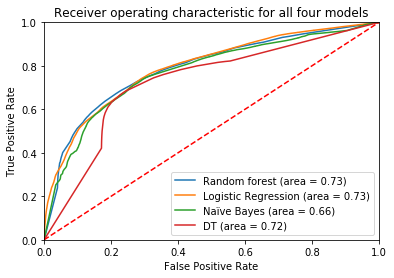
\includegraphics[scale=0.9]{roc}
\end{figure}

All classifiers have an AUC between 0.6 and 0.8, which means that the classification results of the classifier are acceptable and may achieve better performance after we adjust the parameters. In this part, we compare four different models to classify crime into theft crime and battery. The best classifiers are the logistic regression classifier and Random Forest. We identified features that can distinguish theft crime and battery crime.

\begin{figure}[!h]
    \caption{accuracy for all four models}
    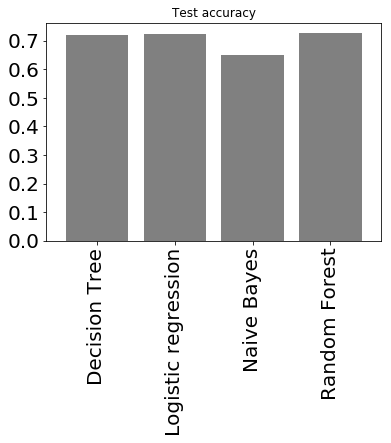
\includegraphics[scale=0.9]{acc}
\end{figure}


\section{Conclusion}
We can see that the most important features determining whether a crime is a theft or not are all indicator variables describing the exact location of the crime (for example if it happened in a department store or apartment, it's will be things like theft). These are consistent with what we predict.

For this study, We only use the Top two crime types(theft and battery). In this case, our classifier based on logistic regression, Random forest, and Decision Tree can reach an accuracy closed to 74$\%$. The classifier based on Naïve Bayes can reach an accuracy closed to 65$\%$.

In the future, we can optimize the performance of the model by adjusting the parameters of the model. And we can classify crime types into severe crimes and less serious crimes so that police stations can allocate police forces. And for some areas, we can prevent certain types of crime by targeting the characteristics of the area. 

We hope this model can show our parents clear information about our safety. If we get the dataset of other cities crimes, we can build another model so that we can find some common characteristics of the type of crime by comparing the model of Chicago and other cities. These common characteristics may help us to build a new common model to predict the crime type for all cities in the United States.

\section{Note}
Abstract, Description and Conclusion part contributed by Haowen. Remain part contributed by Qi.


\bibliography{re}
\bibliographystyle{plain}

\end{document}